%% ------------- Portuguese version ------------
\documentclass{sbrt}
\usepackage[english,brazil]{babel}
\usepackage[utf8]{inputenc}
\usepackage{amsmath,cite}
\usepackage{amssymb}
\usepackage{graphicx}
\usepackage{booktabs}
\graphicspath{{figures/}}
\usepackage[table]{xcolor}
%% ---------------------------------------------
\newcommand{\bblue}[1]{\textcolor{blue}{#1}}
\newcommand{\rred}[1]{\textcolor{red}{#1}}

\begin{document}

\title{Autenticação na Camada Física com Tags Caóticas via Rede Neural: Ablação das Entradas e Núcleo Mínimo em Canal Rayleigh}

\author{Thamires Tavares, Daniel Chaves e Cecílio Pimentel
\thanks{T. Tavares, D.~P.~B. Chaves e C.~J.~L. Pimentel, Departamento de Eletrônica e Sistemas, Universidade Federal de Pernambuco, Recife-PE}%
}


\maketitle

\markboth{XLIV SIMPÓSIO BRASILEIRO DE TELECOMUNICA\c{C}\~{O}ES E PROCESSAMENTO DE SINAIS - SBrT 2026, 29 DE SETEMBRO A 2 DE OUTUBRO DE 2026, SALVADOR, BA}{}


%% ------------- Portuguese version ------------
\begin{resumo}
Este trabalho propõe a aplicação de um discriminador por rede neural ao problema de autenticação na camada física com sequências de autenticação (tags) caóticas em canais Rayleigh. Investigamos três representações de entrada para tomada de decisão do discriminador: (i) um vetor de quatro características fisicamente motivadas, (ii) uma CNN 1D sobre o sinal recebido equalizado após extração da tag legítima ($\mathbf{z}_{eq}$) e (iii) a DNN sobre $\mathbf{z}_{eq}$ . 
Um estudo de ablação sistemático revela o resultado central: apenas dois escalares por pacote — o correlator casado $|\tau|$ e a energia recebida $E$ — são necessários e suficientes para superar o correlator clássico, atingindo $P_D = 87{,}2\%$ a 0~dB contra $8{,}1\%$ do método analítico. Em contrapartida, abordagens baseadas em $\mathbf{z}_{eq}$ falham em baixo SNR por não realizarem integração coerente sem acesso explícito à tag de referência. 

\end{resumo}

\begin{chave}
Autenticação na camada física, discriminador neural, DNN, D3F, CNN 1D, canal Rayleigh, ablação de características, sequências caóticas.
\end{chave}
%% ---------------------------------------------
\rred{Reescrever o abstract e resumo}


\bblue{ (Resumo e abstract reescritos, revisar)}

\begin{abstract}
This paper proposes the application of a neural network discriminator to the problem of physical layer authentication with chaotic authentication sequences (tags) over Rayleigh fading channels. We investigate three input representations for the discriminator's decision-making: (i) a four-feature physically motivated vector, (ii) a 1D CNN over the equalized received signal after legitimate tag extraction ($\mathbf{z}_{eq}$), and (iii) a DNN over $\mathbf{z}_{eq}$.
A systematic ablation study yields the central result: only two scalars per packet — the matched correlator output $|\tau|$ and the received energy $E$ — are necessary and sufficient to outperform the classical correlator, achieving $P_D = 87{,}2\%$ at 0~dB versus $8{,}1\%$ for the analytical method. In contrast, $\mathbf{z}_{eq}$-based approaches fail at low SNR because coherent integration cannot be performed without explicit access to the reference tag.

\end{abstract}
\begin{keywords}
Physical layer authentication, neural discriminator, DNN, D3F, 1D CNN, Rayleigh channel, feature ablation, chaotic sequences.
\end{keywords}

\section{Introdução}

\rred{As referencia devem está na ordem em que são chamadas.}

A autenticação de dispositivos em redes sem fio é um requisito de segurança cada vez mais crítico, especialmente com a expansão de sistemas IoT e 5G/6G~\cite{ref_xie}. Em cenários veiculares (\textit{Vehicle-to-Everything}, V2X)~\cite{ref_3gpp}, por exemplo, dispositivos precisam ser autenticados em dezenas de milissegundos enquanto se deslocam a alta velocidade, uma janela de tempo incompatível com protocolos de troca de chaves convencionais, que exigem múltiplas rodadas de troca de mensagens entre as partes ~\cite{ref_raya}. Abordagens criptográficas tradicionais, implementadas nas camadas superiores da pilha de protocolos, pressupõem capacidade computacional e infraestrutura de gerenciamento de chaves incompatíveis com dispositivos de recursos limitados e com a escala de redes heterogêneas emergentes \rred{referencia, achei a frase forte}. A autenticação na camada física (PLA, \textit{Physical Layer Authentication}) \rred{referencia} surge como solução complementar, explorando características intrínsecas do sinal transmitido — difíceis de reproduzir por adversários sem acesso ao canal legítimo, sem exigir complexidade adicional no receptor. \rred{esta explicação refere-se a PLA passiva. Existe também a PLA ativa que usa tag. }

 \subsection{Definição do Problema}
 
 Dentre as estratégias de PLA, a inserção de sequências de autenticação (tags) caóticas de baixa potência no sinal transmitido destaca-se por combinar sigilo e eficiência~\cite{ref_joao}\rred{Não é bom começar com tag caótica.É melhor colocar a referencia do Yu que propos isto. Deve colocar a tag caótica depois}. Geradas a partir de uma chave secreta compartilhada entre transmissor e receptor, as tags são detectáveis apenas pelo receptor legítimo por meio de correlação com a sequência de referência. O problema de autenticação é então formulado como um teste de hipótese binária entre a presença e a ausência da tag no sinal recebido. Em canais com desvanecimento Rayleigh, no entanto, essa formulação torna-se particularmente desafiadora em baixo SNR, pois o ganho de canal variável altera a distribuição do correlator \rred{correlator ficou meio perdido??}, dificultando a manutenção simultânea de alta probabilidade de detecção e restrição estrita de falso positivo \rred{referencia ??}. Agrava esse cenário o fato de que sistemas práticos exigem probabilidades de falso positivo da ordem de $\alpha = 10^{-7}$, \rred{qual referência ?} cuja verificação direta por Monte Carlo demandaria mais de $10^8$ amostras sob $H_0$ por ponto de operação — tornando a avaliação computacionalmente inviável. \rred{o que é $H_0$ ?} \rred{Qual a importância da avaliação computacional em um sistema prático  ?  }

\rred{ A motivação do artigo está na dificuldade de simulação ? }

\subsection{Solução proposta}

\rred{A seção tem que ser reescrita. }

O \textit{Data-Driven Detection Framework} (D3F)~\cite{ref_braca} contorna esse obstáculo para qualquer classificador neural utilizando a entropia cruzada binária (BCE) como função de perda para determinar os escores de decisão. Isto é implementado por meio do ajuste de uma gaussiana à distribuição desses escores sob $H_0$ a partir de $\sim\!10^3$--$10^4$ amostras; e extrapolação do limiar para $\alpha = 10^{-7}$ por inversão analítica da CDF gaussiana — sem necessitar de $10^8$ simulações. Dois resultados formais de~\cite{ref_braca} validam esse procedimento: (i) a estatística D3F com BCE converge em distribuição para uma gaussiana sob $H_0$; e (ii) os escores D3F convergem ao detector ótimo de Neyman-Pearson — permitindo que qualquer arquitetura com BCE sirva como estatística de teste.

Como metodologia de investigação, este trabalho propõe: (i) aplicação do D3F ao PLA com tags caóticas em Rayleigh, com vetor $\mathbf{f} = [|\tau^i|, \hat{h}, \widehat{\text{SNR}}, E]$ justificado por teoria de detecção; (ii) comparação entre entrada multi-características versus CNN 1D sobre sinal residual; (iii) ablação que identifica o par mínimo $[|\tau|, E]$ como suficiente, atingindo $P_D = 87{,}2\%$ a 0~dB — resultado contraintuitivo que supera a baseline de quatro características.

\section{Fundamentação Teórica}

\subsection{Modelo do Canal e Sinais}

\rred{Não colocar valor particular para 
$L$, $\rho_s$ e $\rho_t$.}

Considera-se um cenário com transmissor legítimo (Alice), receptor (Bob) e atacante (Eve) em canal com desvanecimento  Rayleigh plano e lento~\cite{ref_joao} \rred{esta referência não tem Rayleigh??} . Alice transmite $\mathbf{x}^i = \rho_s \mathbf{s}^i + \rho_t \mathbf{t}^i$, onde $\mathbf{s}^i \in \{-1,+1\}^L$ é a mensagem BPSK e $\mathbf{t}^i$ é a tag caótica, com $\rho_s^2 + \rho_t^2\ =  \mathbb{E}[(t_k^i)^2] = 1$ garantindo potência constante. 

Assume-se que o ganho $h^i$ é constante ao longo de um pacote de $L$ símbolos e varia independentemente entre pacotes com distribuição Rayleigh. Logo, $\mathbb{E}[(h^i)^2] = 1$ e ruído AWGN $\mathbf{w}^i \sim \mathcal{N}(\mathbf{0}, \sigma_w^2\mathbf{I})$.

A SNR instantânea $\gamma^i = (h^i \cdot s^i)^2/\sigma_w^2$ segue distribuição exponencial com média $\bar{\gamma} = 1/\sigma_w^2$, e Bob conhece o estado do canal (\textit{Channel State Information}, CSI).  Neste trabalho, $\rho_s \gg \rho_t$, de modo que o impacto da tag na recuperação da mensagem é mínimo. O sinal recebido por Bob é $\mathbf{y}^i = h^i(\rho_s \mathbf{s}^i + \rho_t \mathbf{t}^i) + \mathbf{w}^i$.

Bob estima $h^i$ pelo estimador de mínimos quadrados~\cite{ref_kay} usando os $L$ símbolos piloto da mensagem: $\hat{h}^i = (\mathbf{s}^i)^\top \mathbf{y}^i / (L \rho_s)$, cujo erro de estimação tem variância $\sigma_e^2 = \sigma_w^2 / (L \rho_s^2)$. A $\overline{\text{SNR}} = 0$~dB e $L = 1024$, obtém-se $\sigma_e^2 \approx 10^{-3}$ — erro desprezível frente ao ganho médio unitário $\mathbb{E}[(h^i)^2] = 1$. \rred{Portanto, a hipótese de CSI perfeito adotada neste trabalho é uma aproximação válida, e os resultados da 4-feat DNN não seriam alterados de forma significativa por estimativas práticas de canal.} - \bblue{Submeter ao escrutínio de uma simulação que reforça a afirmação.}

\subsection{Sinais e o Modelo de Canal}


Considera-se um cenário com transmissor legítimo (Alice), receptor legítimo (Bob) e atacante (Eve) em canal com desvanecimento  Rayleigh plano e lento. 
No $i$-ésimo intervalo de sinalização, Alice transmite $\mathbf{x}^i = \rho_s \mathbf{s}^i + \rho_t \mathbf{t}^i$, em que $\mathbf{s}^i \in \{-1,+1\}^L$ é um vetor de  mensagem de comprimento $L$ contendo símbolos equiprováveis e o vetor $\mathbf{t}^i$ é a tag caótica de comprimento $L$. Os parâmetros $\rho_s$ e
$\rho_t$ determinam a alocação relativa de energia entre a mensagem e a tag. O caso especial $\rho_s=1$ e
$\rho_t=0$ corresponde a uma transmissão sem tag ($\mathbf{x}^i = \mathbf{s}^i)$. 
Para que a energia do sinal transmitido seja igual para o caso com ou sem tag, assume-se que  \rred{$\rho_s^2 + \rho_t^2\ \mathbb{E}[(t_k^i)^2]  = 1$} - \bblue{Informação dada anteriormente}.

 O sinal recebido \rred{por} é $\mathbf{y}^i = h^i(\rho_s \mathbf{s}^i + \rho_t \mathbf{t}^i) + \mathbf{w}^i$.
\rred{Assume-se que o ganho $h^i$, com $\mathbb{E}[(h^i)^2] = 1$,  é constante ao longo de um pacote de $L$ símbolos e varia independentemente entre pacotes com distribuição Rayleigh.
O vetor $\mathbf{w}^i$ é composto de variáveis aleatórias Gaussianas, independentes de média zero e variância $\sigma_w^2$.}
Define-se a relação sinal ruído (SNR, signal to noise ratio ) por
\begin{equation}
\mbox{SNR} = \frac{\mathbb{E}[(h^i)^2] \mathbb{E}[(s^i)^2]}{\sigma_w^2}} = \frac{1}{\sigma_w^2}. 
\end{equation}

%A SNR instantânea $\gamma^i = (h^i \cdot s^i)^2/\sigma_w^2$ segue distribuição exponencial com média $\bar{\gamma} = 1/\sigma_w^2$, e Bob conhece o estado do canal (\textit{Channel State Information}, CSI).  Neste trabalho, $\rho_s \approx 0{,}992$ e $\rho_t \approx 0{,}212$, de modo que o impacto da tag na recuperação da mensagem é mínimo. O sinal recebido por Bob é $\mathbf{y}^i = h^i(\rho_s \mathbf{s}^i + \rho_t \mathbf{t}^i) + \mathbf{w}^i$.

\subsection{Geração de Tags Caóticas}

A tag $\mathbf{t}^i$ é gerada pelo mapa da tenda~\cite{ref_joao}, com condição inicial $x_0 = (\sum_\ell s^i_\ell \oplus k_\ell) \bmod 1$ derivada da mensagem e de uma chave secreta $\mathbf{k} \in \{0,1\}^L$ \bblue{compartilhada entre os usuários legítimos}:\rred{a operação $\oplus$ é entre símbolos de alfabetos distintos.}
\begin{equation}\label{eq:tentmap}
    f(x) = \begin{cases} 2x+1, & x \in [-1,0) \\ 1-2x, & x \in [0,1] \end{cases}
\end{equation}
A alta autocorrelação e baixa correlação cruzada de sequências caóticas com condições iniciais distintas garantem que Bob detecte a tag de Alice \rred{mas não a de Eve — gerada com chave diferente }—, provendo resistência natural a ataques de personificação~\cite{ref_joao}.
\rred{especificar $\mathbb{E}[(t_k^i)^2]$ = ? }.


\subsection{Teste de Hipótese para Autenticação}\label{sec:hip}

O problema \rred{qual ?} é modelado como teste de hipótese binária \rred{em que referência ?}, com $H_0$ indicando ausência de tag (intruso) e $H_1$ indicando presença de tag (autêntico). A estatística de decisão é o correlator casado com a tag~\cite{ref_joao}: \rred{trocar  a referencia} \bblue{Assume-se que o ganho $h^i$ é perfeitamente conhecido pelo receptor}
\begin{equation}\label{eq:tau}
    \tau^i = \left(\frac{\mathbf{y}^i}{h^i} - \rho_s \mathbf{s}^i\right) \cdot \frac{\mathbf{t}^{\mathrm{ref}}}{\rho_t},
\end{equation}
cuja distribuição condicional, pelo Teorema Central do Limite com $L = 1024$, é gaussiana em ambas as hipóteses:
\begin{align}
    \tau^i \mid H_0 &\sim \mathcal{N}\!\left(0,\; \sigma_{v^i}^2\right),\quad
    \tau^i \mid H_1 \sim \mathcal{N}\!\left(|\mathbf{t}^i|^2,\; \sigma_{v^i}^2\right), \label{eq:dists}
\end{align}
onde $\sigma_{v^i}^2 = L\,\mathbb{E}[(t^i_k)^2]/(\rho_t^2\,\gamma^i)$ depende da SNR instantânea.
 A regra de decisão $\tau^i \underset{H_0}{\overset{H_1}{\gtrless}} \tau^i_0$ impõe a restrição de falso positivo:
\begin{equation}\label{eq:alpha}
    \alpha = \Pr(\tau^i > \tau_0^i \mid H_0) = \int_{\tau_0^i}^{\infty} p_{\tau^i|H_0}(\tau)\,d\tau < \eta,
\end{equation}
resultando em $\tau^i_0 = \min\limits_{\tau^i}\,Q^{-1}\!\left(\dfrac{\tau^i}{\sigma^2_{v^i}}\right) < \eta$.


\subsection{Framework D3F e Extrapolação do Limiar}\label{sec:d3f}

O \textit{Data-Driven Detection Framework} (D3F)~\cite{ref_braca} é um método para construir detectores de Neyman-Pearson diretamente a partir de dados, sem conhecimento explícito das distribuições condicionais $p_{\tau|H_0}$ e $p_{\tau|H_1}$. A ideia central é treinar um classificador neural com a entropia cruzada binária (BCE), que incentiva a rede a produzir escores de saída calibrados com probabilidades. O resultado teórico chave de~\cite{ref_braca} é que, sob essa condição de treinamento, os escores se distribuem assintoticamente de forma gaussiana sob $H_0$ — independentemente da arquitetura utilizada.

Essa propriedade permite superar o principal obstáculo prático na avaliação de detectores com restrições severas de falso positivo. Por exemplo: verificar $\alpha$ por simulação direta de Monte Carlo exigiria um número de amostras da ordem de $1/\alpha$ sob $H_0$, tornando a avaliação proibitiva para valores rigorosos de $\alpha$. O D3F substitui essa abordagem exaustiva por duas etapas: (i)~ajusta uma gaussiana $\mathcal{N}(\hat{\mu}_{H_0}, \hat{\sigma}_{H_0}^2)$ à distribuição dos escores sob $H_0$ a partir de apenas ${\sim}\,10^3$--$10^4$ amostras; e (ii)~extrapola analiticamente o limiar para qualquer $\alpha$ desejado, invertendo a função de distribuição acumulada gaussiana:
\begin{equation}\label{eq:d3f}
    \tau^*(\alpha) = \hat{\mu}_{H_0} + \Phi^{-1}(1-\alpha)\,\hat{\sigma}_{H_0},
\end{equation}
reduzindo em ordens de grandeza o custo computacional da avaliação. A probabilidade de detecção é então estimada como a fração de amostras $H_1$ com escore acima de $\tau^*(\alpha)$.

Um segundo resultado de~\cite{ref_braca} fortalece a adoção do D3F: com o crescimento do conjunto de treino, os escores convergem ao teste de razão de verossimilhança de Neyman-Pearson~\cite{ref_poor,ref_veldhuis} — o detector ótimo para uma restrição fixada de $\alpha$. Cabe ressaltar que~\cite{ref_braca} trata observações escalares IID (Independentes e Identicamente Distribuídas) sem engenharia de características; a aplicação do D3F ao cenário de PLA com tags caóticas em canal Rayleigh, com o vetor $\mathbf{f}$ fisicamente motivado, constitui contribuição original deste trabalho.

A hipótese de gaussianidade sob $H_0$ é satisfeita analiticamente para $\tau^i$~\eqref{eq:dists} e empiricamente para a 4-feat DNN bem calibrada com BCE. Para a 1D CNN em baixo SNR, a sobreposição dos escores entre hipóteses torna $\hat{\sigma}_{H_0}$ instável, superestimando $\tau^*$. A Figura~\ref{fig:system} sintetiza o fluxo completo do sistema proposto, desde a transmissão com tag caótica por Alice até a decisão de autenticação por Bob via D3F.

\begin{figure*}[t]
  \centering
  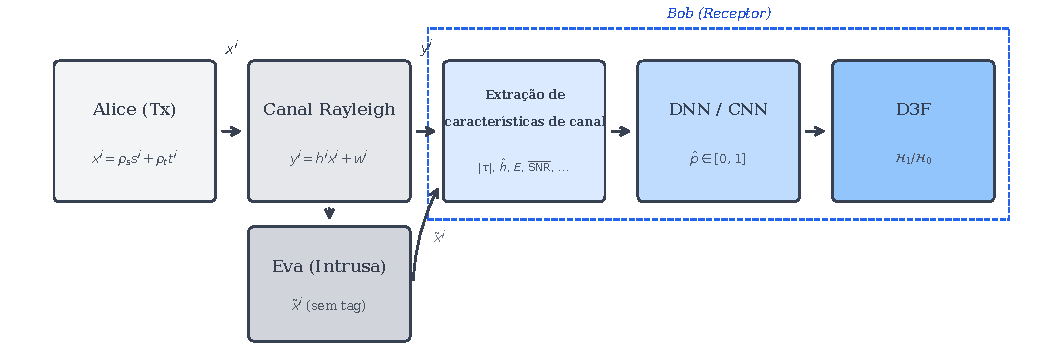
\includegraphics[width=\textwidth]{figures/fig_system_diagram}
  \caption{\label{fig:system}Diagrama do sistema de autenticação na camada física proposto. Alice transmite $x^i = \rho_s s^i + \rho_t t^i$, incorporando a sequência TAG caótica $t^i$. O canal Rayleigh introduz desvanecimento $h^i$ e ruído AWGN $w^i$, produzindo $y^i$ em Bob. O receptor extrai características de canal e as classifica por DNN ou 1D CNN com o framework D3F — gerando o escore $\hat{p} \in [0,1]$ que, comparado ao limiar $\tau^*(\alpha)$~\eqref{eq:d3f}, decide entre $\mathcal{H}_1$ (Alice autêntica) e $\mathcal{H}_0$ (intruso). Eva tenta se autenticar sem possuir a TAG legítima $t^i$.}
\end{figure*}



\section{Métodos Avaliados}

Investigamos o discriminador D3F em três representações de entrada, em ordem crescente de abstração: (i)~vetor de características $\mathbf{f}$ fisicamente motivado (Seção~\ref{sec:dnn4feat}), avaliando também a topologia Dense sobre $\mathbf{z}_{eq}$ como ablação de representação; (ii)~CNN 1D sobre o sinal residual (Seção~\ref{sec:cnn1d}), que testa se o filtro casado pode ser aprendido implicitamente; e (iii)~a mesma CNN com entrada $\mathbf{f}$ para isolar o efeito da arquitetura (Seção~\ref{sec:cnn4feat}). Um SVM linear serve de referência não-neural sobre $\mathbf{f}$ (Seção~\ref{sec:svm}).

\subsection{DNN com Quatro Características (4-feat DNN)}\label{sec:dnn4feat}

A DNN de quatro características recebe como entrada $\mathbf{f} = [|\tau^i|,\, \hat{h},\, \widehat{\text{SNR}},\, E]$, onde $|\tau^i|$ é o módulo do correlator casado~\eqref{eq:tau}, $\hat{h}$ e $\widehat{\text{SNR}}$ são estimativas instantâneas do ganho e da SNR obtidas pelos $L = 1024$ símbolos piloto, e $E = \|\mathbf{y}\|^2/L$ é a energia média do sinal recebido. Cada componente é justificada pela teoria de detecção:

\begin{itemize}
  \item \textbf{$|\tau^i|$}: estatística suficiente do teste de Neyman-Pearson ótimo para o modelo gaussiano de~\eqref{eq:dists}~\cite{ref_poor}; equivale ao filtro casado com a tag~\cite{ref_proakis}, maximizando o SNR de saída.
  \item \textbf{$\hat{h}$ e $\widehat{\text{SNR}}$}: o limiar analítico $\tau_0^i \propto 1/\sqrt{\gamma^i}$ varia de pacote a pacote; fornecer estimativas instantâneas permite à DNN aprender implicitamente o comportamento CFAR~\cite{ref_poor}.
  \item \textbf{$E$}: proporcional à potência recebida, serve como proxy de energia total; sob $H_0$, $E \approx \sigma_w^2$; sob $H_1$, $E$ cresce com $\rho_t^2(h^i)^2$, provendo informação complementar ortogonal a $|\tau^i|$.
\end{itemize}

A topologia adotada é $[4] \to \text{D}(256) \to \text{D}(128) \to \text{D}(64) \to [1]$, onde cada camada D$(n)$ inclui \textit{Batch Normalization}, ReLU e \textit{Dropout} ($p = 0{,}3$). O modelo tem ${\approx}\,44{.}000$ parâmetros treináveis e AUC $= 0{,}9998$. Para verificar se o ganho provém das características ou da arquitetura, treinamos também a \textbf{DNN-1024}: mesma topologia Dense$(256\!\to\!128\!\to\!64)$, mas recebendo $\mathbf{z}_{eq} \in \mathbb{R}^{1024}$ como entrada — sem $|\tau|$ explícito, a tarefa de aprender o filtro casado revela-se inviável abaixo de 15~dB.

\subsection{1D CNN com sinal residual}\label{sec:cnn1d}

A 1D CNN~\cite{ref_liao,ref_oshea} processa diretamente o sinal residual $\mathbf{z}_{eq} \in \mathbb{R}^{1024}$. A motivação é análoga à de um banco de filtros adaptativos: uma camada Conv1D com $c$ filtros de tamanho $k$ equivale a um banco de $c$ filtros FIR de ordem $k$ com coeficientes aprendíveis~\cite{ref_proakis}. A arquitetura adotada é:
\begin{equation}\label{eq:cnn}
\underbrace{[1024,1]}_{\mathbf{z}_{eq}}\!\to\!\text{Conv}_{32}^{15}\!\to\!\text{Conv}_{64}^{9}\!\to\!\text{Conv}_{128}^{5}\!\to\!\text{GAP}\!\to\!\text{D}(64)\!\to\![1],
\end{equation}
onde $\text{Conv}_{c}^{k}$ denota convolução 1D ($c$ filtros, kernel $k$) seguida de BN, ReLU e MaxPooling(4), e GAP é \textit{Global Average Pooling}. O modelo tem ${\approx}\,69{.}000$ parâmetros e AUC $= 0{,}898$.

\subsection{CNN com Quatro Características (CNN-4feat)}\label{sec:cnn4feat}

A CNN-4feat aplica Conv1D sobre o mesmo vetor $\mathbf{f} = [|\tau^i|, \hat{h}, \widehat{\text{SNR}}, E]$:
$[4,1]\!\to\!\text{Conv}_{16}^{2}\!\to\!\text{Conv}_{32}^{2}\!\to\!\text{GAP}(32)\!\to\!\text{D}(16)\!\to\![1]$,
com ${\approx}1{.}000$ parâmetros e AUC $= 0{,}9998$. Ao manter as mesmas entradas e variar apenas a arquitetura, diferenças de desempenho entre CNN-4feat e 4-feat DNN são atribuíveis exclusivamente à topologia — não às características.

\subsection{SVM Linear (referência não-neural)}\label{sec:svm}

Um SVM linear (perda \textit{hinge}, $\lambda = 10^{-4}$, 200 épocas) sobre $\mathbf{f}$ maximiza a margem geométrica entre as classes. Com $|\tau|$ como estatística suficiente analítica, a fronteira de decisão é aproximadamente linear em $\mathbb{R}^4$, tornando o kernel linear adequado e estabelecendo referência não-neural robusta.

\subsection{Protocolo de Treinamento}

Todos os classificadores neurais são treinados por minimização da BCE com o otimizador Adam~\cite{ref_adam} ($\eta_0 = 10^{-3}$, mini-lotes de 512 amostras), \textit{EarlyStopping} (paciência 20 épocas), \textit{ReduceLROnPlateau} (fator 0,5, paciência 10 épocas) e \textit{Dropout} ($p = 0{,}2$ em camadas convolucionais). A BCE incentiva escores calibrados — propriedade essencial para que a distribuição sob $H_0$ seja aproximadamente gaussiana e a extrapolação D3F via~\eqref{eq:d3f} seja válida.


\section{Dataset: Geração e Simulação}

\subsection{Modelo de Sinal e Parâmetros}

O dataset é gerado através de simulação Monte Carlo que reproduz fielmente as condições de canal e modulação. A transmissão autêntica (hipótese $H_1$) segue:
\begin{equation}\label{eq:sig_h1}
\mathbf{y}^i = h^i \left( \rho_s \mathbf{s}^i + \rho_t \mathbf{t}^i \right) + \mathbf{w}^i,
\end{equation}
onde $\rho_s = \sqrt{0{,}985} \approx 0{,}992$ é a amplitude da mensagem BPSK (1024 símbolos), $\rho_t = \sqrt{0{,}015 / 0{,}333} \approx 0{,}212$ é a amplitude da TAG (com normalização $\mathbb{E}[\mathbf{t}^2] \approx 1/3$ proveniente do mapa de tenda), $h^i$ é o ganho Rayleigh, e $\mathbf{w}^i \sim \mathcal{N}(\mathbf{0}, \sigma_w^2 \mathbf{I})$ é ruído AWGN. O ganho satisfaz $\mathbb{E}[(h^i)^2] = 1$, normalizando a potência de transmissão.

A transmissão fraudulenta (hipótese $H_0$) omite a TAG:
\begin{equation}\label{eq:sig_h0}
\mathbf{y}^i = h^i \rho_s \mathbf{s}^i + \mathbf{w}^i,
\end{equation}
refletindo que um atacante sem acesso à chave não pode reproduzir a sequência caótica. Bob estima o canal utilizando a mensagem conhecida e computa o correlator conforme Eq.~\ref{eq:tau}.

\subsection{Estratégia de Amostragem Estratificada}

O dataset é construído com 350.000 amostras balanceadas (175k por classe) distribuídas uniformemente em 6 bins de SNR: $[0,5)$, $[5,10)$, $\ldots$, $[25,30]$~dB. Sobreamostragem é aplicada em baixo SNR ($[0,10)$ dB): fator 1,5× para garantir que o modelo aprenda bem justamente onde a discriminação é mais difícil. Comprimento de mensagem varia em $[512, 1024]$ símbolos, zero-preenchido para 1024 em representação vetorial.

Cada amostra compreende:
\begin{itemize}
  \item $\mathbf{y}_{eq}^i = \mathbf{y}^i / h^i$ — sinal equalizado bruto (referência)
  \item $\mathbf{z}_{eq}^i = \mathbf{y}^i / h^i - \rho_s \mathbf{s}^i$ — resíduo após remoção da mensagem (entrada para CNN/DNN-1024)
  \item $\tau^i$ — correlator clássico (Xie 2021, Eq.~5)
  \item $h^i$, $\text{SNR}^i$ — metadados
  \item Rótulo: $y^i \in \{0, 1\}$
\end{itemize}

Diferença crítica: $\mathbf{z}_{eq}$ isola a TAG da mensagem conhecida. Sob $H_1$: $\mathbf{z}_{eq} = \rho_t \mathbf{t} + \mathbf{w}/h$ (TAG + ruído). Sob $H_0$: $\mathbf{z}_{eq} \approx \mathbf{w}/h$ (ruído puro, pois $(1-\rho_s) \approx 0{,}008 \ll 1$). Esta representação é essencial para redes que aprendem do sinal residual.

\subsection{Particionamento e Normalização}

O dataset de 350k amostras é particionado respeitando estratificação por classe e SNR:
\begin{itemize}
  \item \textbf{Treino} (280k, 80\%): Otimização de parâmetros neurais
  \item \textbf{Validação} (35k, 10\%): Parada antecipada e ajuste de hiperparâmetros
  \item \textbf{Teste} (35k, 10\%): Avaliação final sem viés de treinamento
\end{itemize}

Características são normalizadas globalmente (z-score sobre o conjunto de treino) antes de alimentar as redes densas, garantindo convergência estável. Para a CNN 1D, normalização é aplicada por amostra (remover média e redimensionar cada vetor $\mathbf{z}_{eq}$ independentemente) para não remover informação de amplitude sensível ao SNR.


\section{Resultados e Discussão}

A Figura~\ref{fig:pd_snr} apresenta as curvas de $P_D$ versus SNR sob $\alpha = 10^{-7}$ para todos os métodos avaliados, e a Tabela~\ref{tab:resultados} resume os valores em pontos representativos. Os resultados seguem a hierarquia das representações de entrada: métodos com $|\tau|$ explícito dominam em toda a faixa; métodos baseados em $\mathbf{z}_{eq}$ falham abaixo de 15~dB; e o estudo de ablação revela o par mínimo suficiente.

\begin{figure}[htb]
  \centering
  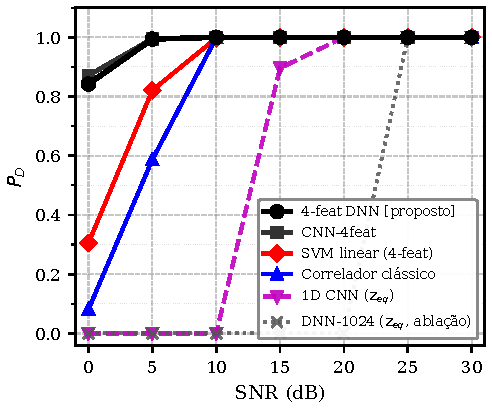
\includegraphics[width=\columnwidth]{figures/fig_pd_snr}
  \caption{\label{fig:pd_snr}$P_D$ vs.\ SNR para todos os métodos avaliados (D3F, $\alpha = 10^{-7}$, $L=1024$, canal Rayleigh). Métodos com $|\tau|$ explícito ultrapassam $P_D = 0{,}8$ a 0~dB; 1D CNN sobre $\mathbf{z}_{eq}$ falha completamente abaixo de 15~dB.}
\end{figure}

\begin{table}[htb]
\caption{\label{tab:resultados}$P_D$ (\%) sob $\alpha = 10^{-7}$ (D3F), $L=1024$, canal Rayleigh. DNN-1024: topologia Dense$(256\!\to\!128\!\to\!64)$ com entrada $\mathbf{z}_{eq}$ (ablação de representação). CNN-4feat: Conv1D sobre as 4 características (ablação de arquitetura).}
\begin{center}
\begin{tabular}{lrrrrrr}\toprule
Método & 0~dB & 5~dB & 10~dB & 15~dB & 20~dB & 25~dB \\\midrule
Clássico~\cite{ref_xie}          &  8{,}1 & 58{,}7 & 99{,}9 & 100{,}0 & 100{,}0 & 100{,}0 \\
\textbf{4-feat DNN}               & \textbf{84{,}2} & \textbf{99{,}4} & \textbf{100{,}0} & \textbf{100{,}0} & \textbf{100{,}0} & \textbf{100{,}0} \\
CNN-4feat                         & 87{,}1 & 99{,}5 & 100{,}0 & 100{,}0 & 100{,}0 & 100{,}0 \\
SVM linear (4-feat)               & 30{,}5 & 82{,}1 & 99{,}7 & 100{,}0 & 100{,}0 & 100{,}0 \\
1D CNN ($\mathbf{z}_{eq}$)~\cite{ref_liao} &  0{,}0 &  0{,}0 &  0{,}0 &  89{,}6 & 100{,}0 & 100{,}0 \\
DNN-1024 ($\mathbf{z}_{eq}$ plano) &  0{,}0 &  0{,}0 &  0{,}0 &   0{,}0 &   0{,}0 &  99{,}8 \\\bottomrule
\end{tabular}
\end{center}
\end{table}

A 4-feat DNN atinge $P_D = 84{,}2\%$ a 0~dB — mais de dez vezes superior ao correlator clássico ($8{,}1\%$) — e $P_D \geq 99{,}4\%$ a partir de 5~dB. O correlator clássico~\cite{ref_xie} falha em baixo SNR porque precisa estimar $\sigma_{v^i}$ com precisão sob desvanecimento severo; a DNN contorna esse problema aprendendo limiares adaptativos por bin de SNR a partir dos dados. A CNN-4feat, com a mesma entrada $\mathbf{f}$ mas arquitetura convolucional, atinge $P_D = 87{,}1\%$ a 0~dB — ligeiramente superior à 4-feat DNN —, confirmando que o desempenho é determinado pelas características de entrada, não pela escolha de arquitetura. O SVM linear com $\mathbf{f}$, apesar de sua fronteira linear, supera ambas as abordagens baseadas em $\mathbf{z}_{eq}$ em toda a faixa avaliada, evidenciando que a representação de entrada domina sobre a expressividade do classificador.

As abordagens baseadas em $\mathbf{z}_{eq}$ revelam uma limitação estrutural comum: sem $|\tau|$ explícito, qualquer arquitetura precisaria aprender o filtro casado implicitamente, tarefa inviável quando $\rho_t \approx 0{,}212$ encobre a TAG em apenas ${\approx}\,4{,}5\%$ da potência total. A 1D CNN falha abaixo de 15~dB ($P_D = 0$) e a DNN-1024 é eficaz apenas a 25~dB ($P_D = 99{,}8\%$), com AUC $= 0{,}718$. Os resultados estabelecem uma hierarquia determinada pela representação: métodos com $|\tau|$ explícito dominam independentemente da arquitetura; métodos baseados em $\mathbf{z}_{eq}$ são ineficazes abaixo de 15~dB por razão estrutural, não por limitação de capacidade.

\subsection{Ablação das Características: Descoberta do Núcleo Mínimo}

Para isolar a contribuição individual de cada característica, treinamos oito variantes da 4-feat DNN mantendo arquitetura e hiperparâmetros inalterados e variando apenas a composição da entrada (Tabela~\ref{tab:feat_ablation}, Figura~\ref{fig:ablation_pd_snr}).

\begin{table}[htb]
\caption{\label{tab:feat_ablation}Ablação de características — $P_D$ (\%) sob $\alpha = 10^{-7}$. Todas as variantes usam a topologia Dense$(256\!\to\!128\!\to\!64)$.}
\begin{center}
{\footnotesize
\begin{tabular}{lrrrrr}\toprule
Variante & 0~dB & 5~dB & 10~dB & 15~dB & 20~dB \\\midrule
Clássico: $|\tau|$ (limiar analítico)            &  8{,}1 & 58{,}7 & 99{,}9 & 100 & 100 \\\midrule
V1: $[|\tau|,\hat{h},\overline{\text{SNR}},E]$   & 82{,}3 & 99{,}5 & 100 & 100 & 100 \\
V2: $h$ perfeito                                 & 83{,}6 & 99{,}5 & 100 & 100 & 100 \\
V3: sem $\overline{\text{SNR}}$                  & 82{,}0 & 99{,}5 & 100 & 100 & 100 \\
V4: sem $E$                                      & 82{,}2 & 99{,}5 & 100 & 100 & 100 \\
V5: $[|\tau|]$ isolado                           &  0{,}0 & 98{,}9 & 100 & 100 & 100 \\\midrule
V6: $[|\tau|,\hat{h}]$                           & 85{,}6 & 99{,}6 & 100 & 100 & 100 \\
V7: $[|\tau|,\overline{\text{SNR}}]$             & 33{,}0 & 99{,}1 & 100 & 100 & 100 \\
\textbf{V8}: $\boldsymbol{[|\tau|,E]}$           & \textbf{87{,}2} & \textbf{99{,}5} & 100 & 100 & 100 \\\bottomrule
\end{tabular}
}
\end{center}
\end{table}

\begin{figure}[htb]
  \centering
  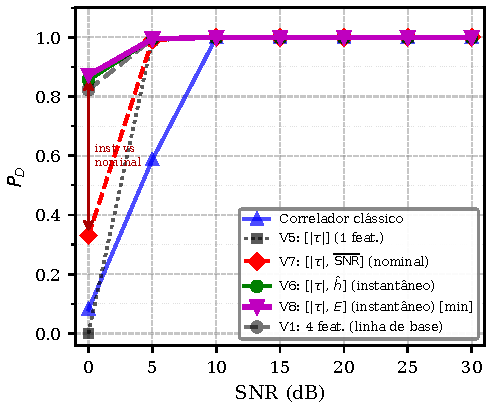
\includegraphics[width=\columnwidth]{figures/fig_ablation_pd_snr}
  \caption{\label{fig:ablation_pd_snr}$P_D$ vs.\ SNR para as variantes de ablação (D3F, $\alpha=10^{-7}$). V7 ($|\tau|$ + SNR nominal) atinge apenas $33\%$ a 0~dB; V8 ($|\tau|$ + energia instantânea) chega a $87{,}2\%$ — superando a linha de base de quatro características (V1, $82{,}3\%$). A seta indica a diferença de $54$~pp atribuível à substituição da SNR nominal pela energia instantânea.}
\end{figure}

\textbf{Fato~1 — CSI perfeito é dispensável.} Substituir $\hat{h}$ por $h$ perfeito (V2) altera $P_D$ em apenas $+1{,}3$~pp a 0~dB. Com $L = 1024$ símbolos piloto, o estimador de mínimos quadrados produz erro de estimação $\sigma_e^2 \approx 10^{-3}$~\cite{ref_kay}, tornando a hipótese de CSI perfeito uma aproximação válida na prática.

\textbf{Fato~2 — Características auxiliares são coletivamente necessárias, mas individualmente redundantes.} Remover qualquer uma delas (V3, V4) impacta $P_D$ em no máximo $-0{,}3$~pp; remover todas (V5) produz $P_D = 0$ a 0~dB. Sem nenhuma âncora de escala, a DNN não dispõe de informação sobre o nível instantâneo de ruído — o mesmo problema que impede o correlator clássico de atingir $P_D > 50\%$ a 0~dB.

\textbf{Fato~3 — A informação instantânea é determinante.} V6~$[|\tau|, \hat{h}]$ e V8~$[|\tau|, E]$ superam o correlator clássico com apenas 2 escalares por pacote, atingindo $P_D \geq 85\%$ a 0~dB. V8 atinge $87{,}2\%$ — \emph{superior à linha de base de quatro características} (V1, $82{,}3\%$) —, evidenciando que a capacidade representacional concentrada em dois graus de liberdade informativos supera a de uma rede com quatro entradas parcialmente redundantes. Em contraste, V7~$[|\tau|, \overline{\text{SNR}}]$ atinge apenas $33{,}0\%$, apesar de também usar 2 características. A diferença é estrutural: $\hat{h}$ e $E$ são calculados \emph{por pacote} — refletindo o ganho instantâneo $h^i$ — enquanto $\overline{\text{SNR}}$ é o rótulo médio do bin, insensível às flutuações de $h^i$ dentro do bin. Sob desvanecimento Rayleigh, a variância intra-bin de $h^i$ é da mesma ordem que a variância inter-bin; portanto, a SNR nominal retém muito menos informação sobre $\sigma_{v^i}^2 \propto 1/(h^i)^2$ do que qualquer estimativa instantânea. Esse resultado fornece justificativa experimental para o princípio CFAR~\cite{ref_poor}: o limiar deve adaptar-se ao \emph{nível de ruído da amostra corrente}, não à média do regime.

O número mínimo de características para superar o correlator clássico é, portanto, \textbf{dois}: $|\tau|$ (estatística suficiente do teste NP) mais uma estimativa instantânea do canal ($\hat{h}$ ou $E$), ambas computáveis com custo $\mathcal{O}(L)$ a partir do sinal recebido.


\section{Conclusões}

Este trabalho apresentou a primeira aplicação de um discriminador neural orientado a dados (D3F) ao problema de autenticação na camada física com tags caóticas em canal Rayleigh, avaliando sistematicamente três representações de entrada sob $\alpha = 10^{-7}$. A investigação seguiu um caminho lógico: partindo do vetor de quatro características fisicamente motivadas, passando pela CNN 1D sobre o sinal residual, até a ablação sistemática das entradas. O resultado central é contraintuitivo: \textbf{o melhor desempenho é obtido com apenas duas características} — o correlator casado $|\tau|$ e a energia instantânea $E$ —, com $P_D = 87{,}2\%$ a 0~dB, superando tanto o correlator clássico ($8{,}1\%$) quanto a linha de base de quatro características ($82{,}3\%$). A explicação é estrutural: abordagens baseadas em $\mathbf{z}_{eq}$ (1D CNN e DNN-1024) falham abaixo de 15~dB porque, sem $|\tau|$ explícito, não há como realizar integração coerente quando $\rho_t \approx 0{,}212$ encobre a TAG no ruído. O estudo de ablação confirma que as características auxiliares $\hat{h}$ e $\overline{\text{SNR}}$ são individualmente redundantes e que a chave do desempenho é a distinção entre informação \emph{instantânea} ($\hat{h}$, $E$) e nominal ($\overline{\text{SNR}}$): $[|\tau|, E]$ supera $[|\tau|, \overline{\text{SNR}}]$ em 54~pp a 0~dB, validando o princípio CFAR. Esses resultados estabelecem o par $[|\tau|, E]$ como o núcleo discriminatório mínimo e suficiente para autenticação robusta em canal Rayleigh.

Trabalhos futuros investigarão funções de perda que regularizem diretamente a distribuição de escores sob $H_0$ — como perda focal ou restrições sobre momentos de ordem superior — e a extensão da abordagem a canais veiculares (V2V/V2X)~\cite{ref_3gpp}, onde a variação rápida de $h^i$ exige estimativas de canal mais robustas e representa aplicação natural para os classificadores orientados a dados aqui avaliados.

\section*{Agradecimentos}
Os autores agradecem ao Departamento de Eletrônica e Sistemas da Universidade Federal de Pernambuco pelo apoio na realização deste trabalho.

\section*{Lista de Siglas}
{\small
\begin{tabular}{@{}p{1.9cm}p{5.9cm}@{}}
\textbf{1D CNN}    & \textit{One-Dimensional Convolutional Neural Network} \\
\textbf{AWGN}      & \textit{Additive White Gaussian Noise} \\
\textbf{BCE}       & \textit{Binary Cross-Entropy} (Entropia Cruzada Binária) \\
\textbf{BN}        & \textit{Batch Normalization} \\
\textbf{BPSK}      & \textit{Binary Phase Shift Keying} \\
\textbf{CFAR}      & \textit{Constant False Alarm Rate} (Taxa Constante de Falso Positivo) \\
\textbf{CNN}       & \textit{Convolutional Neural Network} \\
\textbf{CSI}       & \textit{Channel State Information} \\
\textbf{D3F}       & \textit{Data-Driven Detection Framework}~\cite{ref_braca} \\
\textbf{DNN}       & \textit{Deep Neural Network} \\
\textbf{GAP}       & \textit{Global Average Pooling} \\
\textbf{IoT}       & \textit{Internet of Things} \\
\textbf{LRT}       & \textit{Likelihood Ratio Test} \\
$\boldsymbol{P_D}$ & Probabilidade de Detecção \\
\textbf{PLA}       & \textit{Physical Layer Authentication} \\
\textbf{ReLU}      & \textit{Rectified Linear Unit} \\
\textbf{SNR}       & \textit{Signal-to-Noise Ratio} \\
\textbf{SVM}       & \textit{Support Vector Machine} \\
\textbf{TCL}       & Teorema Central do Limite \\
\end{tabular}
}

\begin{thebibliography}{99}

\bibitem{ref_xie} H. Xie, W. Chen, e J. Ning, ``Security Model of Authentication at the Physical Layer and Performance Analysis over Fading Channels,'' \textit{IEEE Trans.\ Inf.\ Forensics Security}, v.~16, pp.~3945--3959, 2021.

\bibitem{ref_braca} P. Braca, S. Marano, V. Matta, e P. Willett, ``Statistical Hypothesis Testing Based on Machine Learning: Large Deviations Analysis,'' \textit{IEEE Open J.\ Signal Process.}, v.~3, pp.~464--484, 2022.

\bibitem{ref_liao} L. Liao, O. Wijesinghe, J. Perez-Ramirez, A. Bhatt, B. Imtiaz, e K. Ding, ``Deep Learning for Wireless Communications,'' \textit{Sensors}, v.~19, n.~11, p.~2440, 2019.

\bibitem{ref_oshea} T. J. O'Shea e J. Hoydis, ``An Introduction to Deep Learning for the Physical Layer,'' \textit{IEEE Trans.\ Cogn.\ Commun.\ Netw.}, v.~3, n.~4, pp.~563--575, 2017.

\bibitem{ref_joao} J. V. C. Evangelista, D. Moreno, D. P. B. Chaves e C. Pimentel, ``Tag Generation Using Chaotic Sequences for Physical-Layer Authentication,'' \textit{IEEE Access}, v.~11, pp.~73080--73087, 2023.

\bibitem{ref_poor} H. V. Poor, \textit{An Introduction to Signal Detection and Estimation}, 2.~ed. Springer-Verlag, 1994.

\bibitem{ref_adam} D. P. Kingma e J. Ba, ``Adam: A Method for Stochastic Optimization,'' em \textit{Proc.\ Int.\ Conf.\ Learn.\ Represent.\ (ICLR)}, San Diego, CA, EUA, 2015.

\bibitem{ref_goodfellow} I. Goodfellow, Y. Bengio e A. Courville, \textit{Deep Learning}. MIT Press, 2016. Disponível em: \texttt{https://www.deeplearningbook.org}.

\bibitem{ref_proakis} J. G. Proakis e D. G. Manolakis, \textit{Digital Signal Processing: Principles, Algorithms, and Applications}, 4.~ed. Pearson Prentice Hall, 2007.

\bibitem{ref_3gpp} 3GPP, ``Study on Channel Model for Frequencies from 0.5 to 100 GHz,'' Technical Report TR 38.901, v17.0.0, 3rd Generation Partnership Project, 2022.

\bibitem{ref_shlezinger} N. Shlezinger, N. Farsad, Y.~C. Eldar e A.~J. Goldsmith, ``Model-Based Machine Learning for Communications,'' arXiv:2101.04726, 2021.

\bibitem{ref_veldhuis} R. Veldhuis e D. Zeng, ``On Neyman-Pearson Optimality of Binary Neural Net Classifiers,'' Tech.\ Rep., jun.\ 2021. DOI: 10.36227/techrxiv.14709930.v1.

\bibitem{ref_kay} S. M. Kay, \textit{Fundamentals of Statistical Signal Processing, Vol.~I: Estimation Theory}. Prentice Hall, 1993.

\bibitem{ref_raya} M. Raya e J.-P. Hubaux, ``Securing Vehicular Ad Hoc Networks,'' \textit{J. Comput. Secur.}, v.~15, n.~1, pp.~39--68, 2007.

\end{thebibliography}

\end{document}
